
%%%%%%%%%%%%%%%%%%%%%%%%%%%%%%%%%%%%%%%%%%%%%%%%%%%%%%%%%%%%

%&latex
\documentclass[12pt]{article}
\usepackage[USenglish]{babel}
\usepackage{graphicx}
\usepackage{bm}
\usepackage{setspace}
\usepackage{varioref}
\usepackage{booktabs}
\usepackage{rotating}
\usepackage{xfrac}
\usepackage{adjustbox}
\usepackage[normalem]{ulem}
\usepackage{longtable} % use for tables going over more than one page
\usepackage{ragged2e}
\usepackage[osf,sc]{mathpazo} % Use the Palatino font
%\usepackage[T1]{fontenc} % Use 8-bit encoding that has 256 glyphs
%\linespread{1.05} % Line spacing - Palatino needs more space between lines
\linespread{1.25} % Line spacing - Palatino needs more space between lines
\usepackage{microtype} % Slightly tweak font spacing for aesthetics
%\usepackage[hmarginratio=1:1,top=32mm,columnsep=20pt]{} %old margins
\usepackage[left=0.93in,right=0.93in,bottom=0.93in,top=0.93in]{geometry} % Document margins
%\usepackage{multicol} % Used for the two-column layout of the document
\usepackage[hang, small,labelfont=bf,up,textfont=it,up]{caption} % Custom captions under/above floats in tables or figures
\usepackage{booktabs} % Horizontal rules in tables
\usepackage{float} % Required for tables and figures in the multi-column environment - they need to be placed in specific locations with the [H] (e.g. \begin{table}[H])	
\usepackage[colorlinks=false]{hyperref}
\usepackage[svgnames]{xcolor}
\hypersetup{colorlinks, citecolor=NavyBlue, urlcolor=NavyBlue, linkcolor=NavyBlue} % For hyperlinks in the PDF
\usepackage{lettrine} % The lettrine is the first enlarged letter at the beginning of the text
\usepackage{paralist} % Used for the compactitem environment which makes bullet points with less space between them
\usepackage{enumitem} 
\usepackage{amsfonts}
\usepackage{amsmath}
\usepackage{amsthm}
\usepackage{mathtools}

% Table sizing
\usepackage{tabularx,ragged2e,booktabs}
\newcolumntype{L}{>{\RaggedRight\arraybackslash}X}
\newcolumntype{C}{>{\centering\arraybackslash}X}
 
  
\theoremstyle{definition}
\newtheorem{definition}{Definition}
\newtheorem{assumption}{Assumption}

\usepackage{sub caption} %allows combination of figures
\usepackage{abstract} % Allows abstract customization
\renewcommand{\abstractnamefont}{\normalfont\bfseries} % Set the "Abstract" text to bold
%\renewcommand{\abstracttextfont}{\normalfont\small\itshape} % Set the abstract itself to small italic text
\usepackage{url}
\usepackage{titlesec} % Allows customization of titles
%\renewcommand\thesection{\Roman{section}} % Roman numerals for the sections
%\renewcommand\thesubsection{\Roman{subsection}} % Roman numerals for subsections
\titleformat{\section}[block]{\large\scshape\centering}{\thesection.}{1em}{} % Change the look of the section titles
\titleformat{\subsection}[block]{\large}{\thesubsection.}{1em}{} % Change the look of the section titles
\usepackage{fancyhdr} % Headers and footers
%\pagestyle{fancy} % All pages have headers and footers
%\fancyhead{} % Blank out the default header
%\fancyfoot{} % Blank out the default footer
%\fancyfoot[RO,LE]{\thepage} % Custom footer text

%\usepackage[left=.25in,right=.25in,top=.25in,bottom=.25in,verbose]{geometry}
\usepackage{booktabs}
\usepackage{pdflscape}


\def\sym#1{\ifmmode^{#1}\else\(^{#1}\)\fi}
\usepackage{rotating,booktabs}
\def\MC#1{\multicolumn{1}{c}{#1}}
\def\ML#1{\multicolumn{1}{l}{#1}}

%\usepackage[longnamesfirst]{natbib}
%\renewcommand*\&{and}
%\bibliographystyle{authordate1}
%\usepackage{authblk}
%\usepackage[super, sort]{natbib}
\usepackage[]{natbib}
\bibliographystyle{chicago_v2}


\usepackage{tikz}
\usetikzlibrary{snakes}
\usepackage{makeidx}
\usepackage{pst-all}
\usepackage{latexsym}
\usepackage{ifthen}
\usepackage{setspace}
\usepackage{pstricks}
\usepackage{pstricks-add}
\usepackage{theorem}
\usepackage{epsfig}
\usepackage{rotating}
\usepackage{lscape}
\usepackage{eurosym}
\usepackage{hyperref}  

\newcommand{\appendixpagenumbering}{
  \break
  \pagenumbering{arabic}
  \renewcommand{\thepage}{A-\arabic{page}}
}

\usepackage{bbm}  

\usepackage{afterpage}  

\usepackage[italic]{mathastext}

% align tables on decimals with siunitx
\usepackage{siunitx}
\sisetup{ detect-all }

%%%%%%%%%%%%%%%%%%%%%%%%%%%%%%%%%%%%%%%%%%%%%%%%%%%%%%%%%%%%

\makeatletter
\def\input@path{%
{xxx/xxx/}%
}
\makeatother
\graphicspath{%
{xxx/xxx/}%
}
\usepackage{caption}



%%%%\makeatletter
%%%%\def\input@path{{../tables/}}
%%%%\makeatother
%%%%
%%%%\graphicspath{{../graphs/}}
%%%%
%%%%
%%%%\usepackage{caption}
%%%%
%%%%\captionsetup[table]{labelformat=empty}
%%%%\captionsetup[figure]{labelformat=empty}


%%%%%%%%%%%%%%%%%%%%%%%%%%%%%%%%%%%%%%%%%%%%%%%%%%%%%%%%%%%%

%\usepackage[ansinew]{inputenc}
\bibpunct{(}{)}{;}{a}{,}{,}
%Umlaute-Paket
%\usepackage[ansinew]{inputenc}
%\bibliographystyle{Econometrica}


%%%%%%%%%%%%%%%%%%%%%%%%%%%%%%%%%%%%%%%%%%%%%%%%%%%%%%%%%%%%

% adjust font inside tabular to cope with input .tex files with tables

\usepackage{etoolbox}% http://ctan.org/pkg/etoolbox
\BeforeBeginEnvironment{tabular}{\small}% Adjust tabular font size to \Huge

%%%%%%%%%%%%%%%%%%%%%%%%%%%%%%%%%%%%%%%%%%%%%%%%%%%%%%%%%%%%
%%%%%%%%%%%%%%%%%%%%%%%%%%%%%%%%%%%%%%%%%%%%%%%%%%%%%%%%%%%%
%%%%%%%%%%%%%%%%%%%%%%%%%%%%%%%%%%%%%%%%%%%%%%%%%%%%%%%%%%%%
%%%%%%%%%%%%%%%%%%%%%%%%%%%%%%%%%%%%%%%%%%%%%%%%%%%%%%%%%%%%

\begin{document}

%
\begin{figure}[b!]
	\caption{LP bias in SMALL samples, $T=100, \rho=0.95 \text{ or }  1, Nreps = 10,000$}
	\label{basicLP_wcbb}

\footnotesize 

True DGP:	\qquad	$y_t =  \rho y_{t-1} + u_t$, \qquad $u \sim N(0,1), \;\; \rho=0.95 \text{ or }  1, \;\;  T=100$ 

Estimated OLS models:

Intercept: no 	 	\qquad	$y_t =  \beta_1 y_{t-1} + u_t$

Intercept: yes	 	\qquad	$y_t =  \beta_1 y_{t-1} + \beta_0 + u_t$

\bigskip

\centering\scriptsize	

 \vspace{1em}

	{\centering%
	\begin{subfigure}{0.5\textwidth}%	
		\caption{$\rho=0.95$; Intercept: no }\includegraphics[width=\textwidth]{"SSBias_IntcpNLagdiffN_rho_950_reps_10000_obs_100.pdf"}%
	\end{subfigure}%
	\begin{subfigure}{0.5\textwidth}%	
		\caption{$\rho=0.95$; Intercept: yes }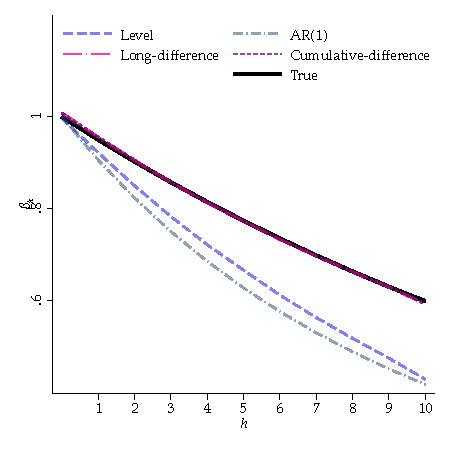
\includegraphics[width=\textwidth]{SSBias_IntcpYLagdiffN_rho_950_reps_10000_obs_100.pdf}%
	\end{subfigure}%
\par
	\begin{subfigure}{0.5\textwidth}%	
		\caption{$\rho=1$; Intercept: no }\includegraphics[width=\textwidth]{"SSBias_IntcpNLagdiffN_rho_1000_reps_10000_obs_100.pdf"}%
	\end{subfigure}%
	\begin{subfigure}{0.5\textwidth}%	
		\caption{$\rho=1$; Intercept: yes }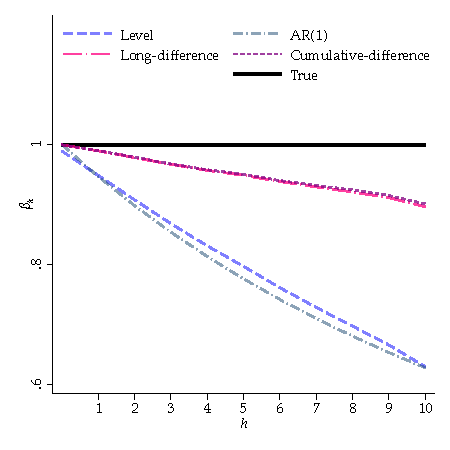
\includegraphics[width=\textwidth]{SSBias_IntcpYLagdiffN_rho_1000_reps_10000_obs_100.pdf}%
	\end{subfigure}%
	}
	
\end{figure}

\newpage


%
\begin{figure}[t!]
	\caption{LP bias in LARGE samples, $T=100,000, \rho=0.95 \text{ or }  1, Nreps = 100$}
	\label{basicLP_wcbb}
	
\footnotesize 

True DGP:	\qquad	$y_t =  \rho y_{t-1} + u_t$, \qquad $u \sim N(0,1), \;\; \rho=0.95 \text{ or } 1, \;\;  T=100,000$ 

Estimated OLS models:

Intercept: no 	 	\qquad	$y_t =  \beta_1 y_{t-1} + u_t$

Intercept: yes	 	\qquad	$y_t =  \beta_1 y_{t-1} + \beta_0 + u_t$

\bigskip

\centering\scriptsize	
 \vspace{1em}

	{\centering%
	\begin{subfigure}{0.5\textwidth}%	
		\caption{$\rho=0.95$; Intercept: no }\includegraphics[width=\textwidth]{"SSBias_IntcpNLagdiffN_rho_950_reps_100_obs_100000.pdf"}%
	\end{subfigure}%
	\begin{subfigure}{0.5\textwidth}%	
		\caption{$\rho=0.95$; Intercept: yes }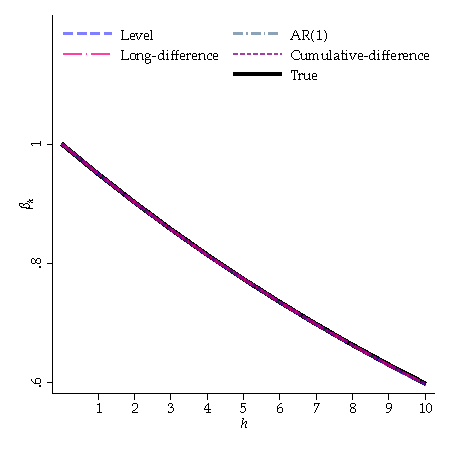
\includegraphics[width=\textwidth]{SSBias_IntcpYLagdiffN_rho_950_reps_100_obs_100000.pdf}%
	\end{subfigure}%
\par
	\begin{subfigure}{0.5\textwidth}%	
		\caption{$\rho=1$; Intercept: no }\includegraphics[width=\textwidth]{"SSBias_IntcpNLagdiffN_rho_1000_reps_100_obs_100000.pdf"}%
	\end{subfigure}%
	\begin{subfigure}{0.5\textwidth}%	
		\caption{$\rho=1$; Intercept: yes }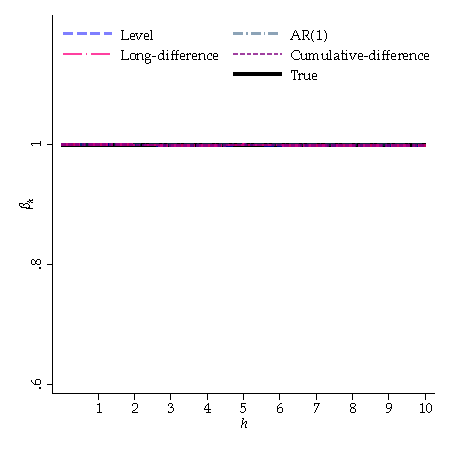
\includegraphics[width=\textwidth]{SSBias_IntcpYLagdiffN_rho_1000_reps_100_obs_100000.pdf}%
	\end{subfigure}%
	}
	
\end{figure}


\end{document}

